\chapter{Testing and Evaluation}

\label{chapter:evaluation}

In this chapter, we outline how the testing and evaluation of the proxy is
performed and present the results obtained. The goal is to validate that the
proxy fulfills the premises and requirements and to measure any possible
improvements (or deteriorations) of the performance of Web services. Based on
the measurements we then give a recommendation about which adaptations to make
in different types of DIL networks. Since the proxy is being developed as a
prototype for military usage, we use test scenarios that resemble actual
military usage. We also included one civilian usage based on \gls{edge} since
civilian mobile phone technology is currently being considered for military use
both by NATO and several nations. For the purpose of testing, we develop two
sets of test applications, one W3C Web service, and one RESTful Web service.
These applications are then used to test the proxy in networks with different
DIL characteristics.

We start this chapter by introducing different types of DIL networks we can
encounter working with tactical networks. Then we present how these networks can
be emulated using the Linux network traffic tools before we introduce evaluation
tools and the two test applications. Next, we put the proxy to the test in an
unlimited network to verify that it behaves correctly. We call this the function
test. Then we start introducing the DIL characteristics into the tests and
measure if we can improve the performance by using proxies. We introduce the
\textit{disconnected} and \textit{intermittent} aspects first before we test the
proxy in six different \textit{limited} networks. We also test in a setup using
actual military communication equipment. This testing was done to validate the
results from the software emulated networks.

Finally, we discuss the results, their underlying causes, and which implications
they have. Ultimately, we give a recommendation about the usage of proxies in
DIL networks.

\section{Types of DIL Networks}

Military communication can occur over a wide range of different technologies and
environments. An infinite number of possible network combinations exist, so we
have chosen to focus on five different network types identified by the task
group IST-118 for DIL-testing \cite{johnsen-recommendations}. The networks were
identified because they represent typical networks typically found in military
communication.  These include \gls{satcom}, \gls{los}, \gls{cnr} and WiFi. WiFi
is divided into two types, one indicating operation in the "sweet spot" and one
in the edge of the network. Some communication technologies, such as satellite
communication, are characterized by long communication delay while others may be
by their low data rate. An overview of selected military communication
technologies can be seen in \cref{figure-networks-overview}.

\begin{figure}[h]
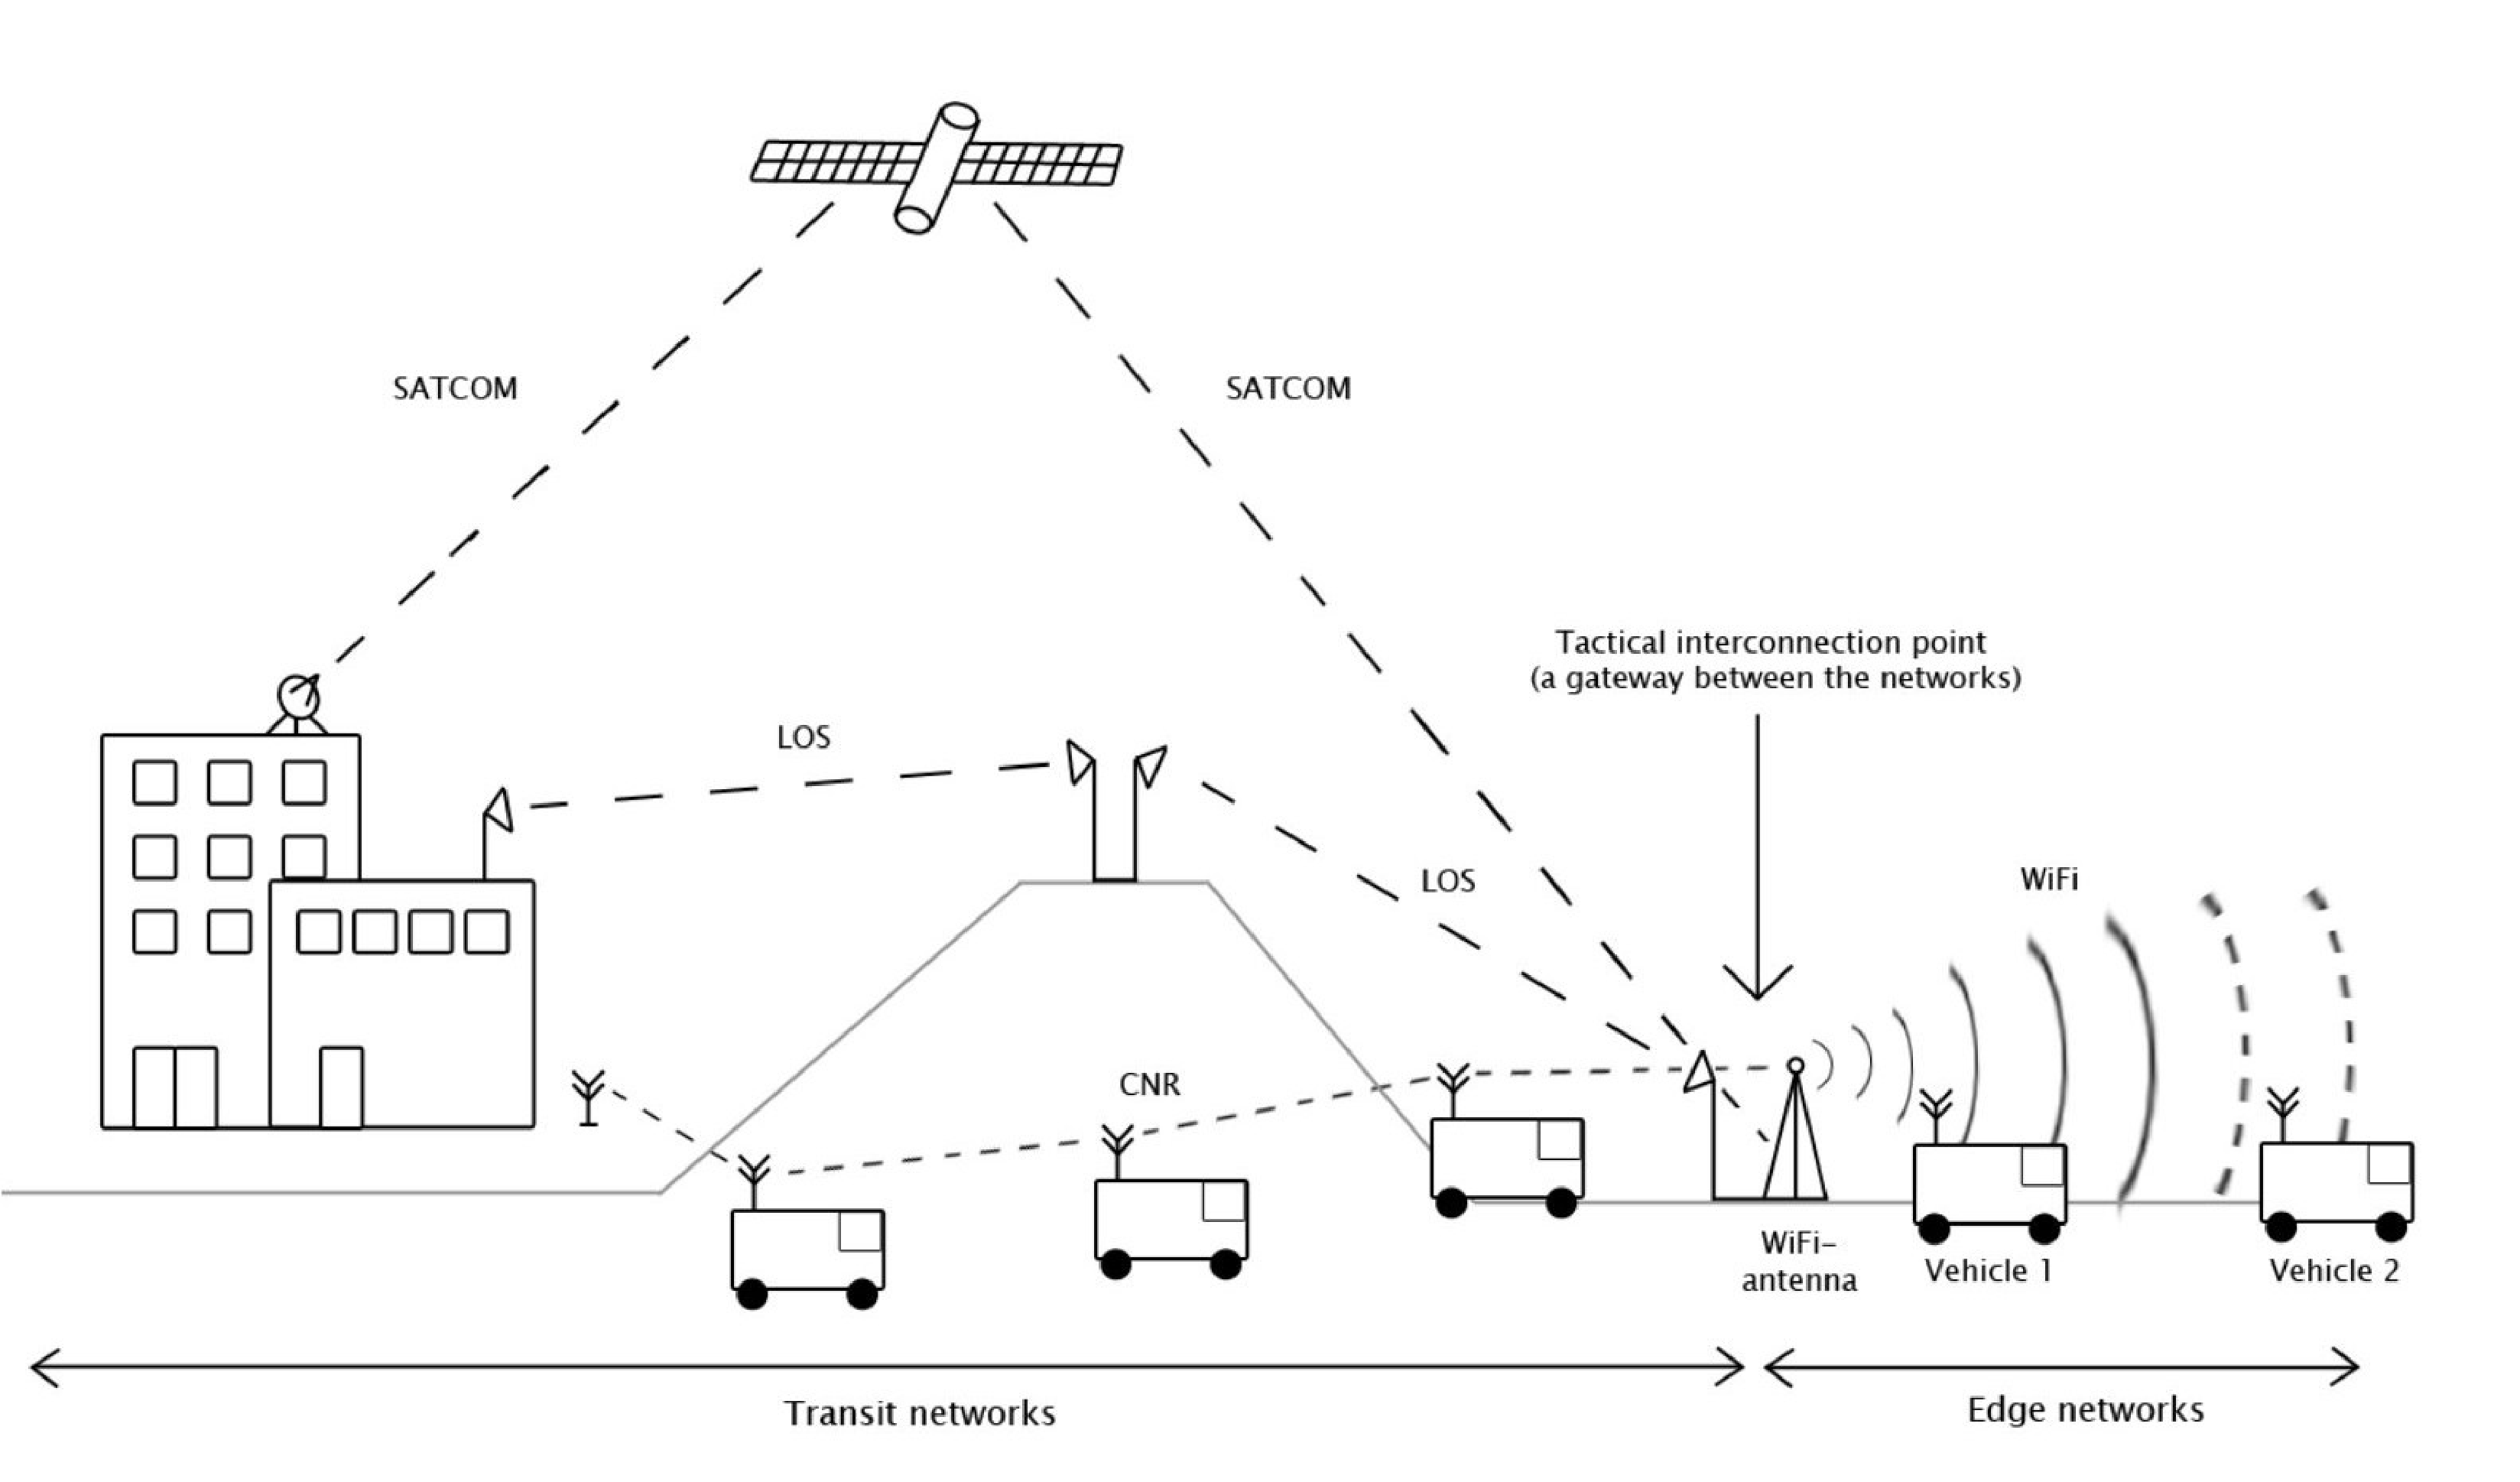
\includegraphics[width=\textwidth]{images/networks_overview.pdf}
\caption{Overview of tested networks (from \cite{krog-pisa})}
\label{figure-networks-overview}
\end{figure}

We also investigated \gls{lte}, commonly known as 4G, a network technology which
has become in widespread use in the latest years. The reason for including LTE
in addition to the ones from IST-118 is that the Norwegian Defense is looking
into the possibility of using LTE. This fact makes it interesting for us to
investigate the performance of Web services in this type of network as well.
However, LTE has gotten so fast and reliable that it is not really relevant from
a DIL perspective. We therefore instead looked into \gls{edge}, which is used as
a fallback in geographical areas where \gls{lte} and 3G are not available. Of
the networks we evaluate for, EDGE is the only one with asymmetrical down- and
upload speed: 50 kbps up and 200 kbps down
\cite{evaluation-transport-protocols-web-services}.

\Cref{table-network-types} summarizes the identified networks and their
propererties.

\begin{table}[h]
\begin{tabular}{| l | l | l | l | l |}
\hline
  \textbf{Network} & \textbf{Data Rate} & \textbf{Delay} & \textbf{PER} \\ \hline
  \gls{satcom} & 250 kbps & 550 ms & 0 \% \\ \hline
  \gls{los} & 2 mbps & 5 ms & 0 \% \\ \hline
  WiFi 1 & 2 mbps & 100 ms & 1 \% \\ \hline
  WiFi 2 & 2 mbps & 100 ms & 20 \% \\ \hline
  \gls{cnr} & 9.6 kbps & 100 ms & 1 \% \\ \hline
  \gls{edge} & 50 kbps up/200 kbps down & 200 ms & 0 \% \\ \hline
\end{tabular}
\caption{Different network types}
\label{table-network-types}
\end{table}


\section{Testing and Evaluation Tools}

To evaluate how using the proxies impacts the performance of Web services in DIL
environments, we needed some way of emulating limited and constrained networks.
Obviously, we would have got the most realistic test environment by testing "out
in the field" ourselves. However, this would require a considerable amount of
effort, and it would be difficult to reproduce the exact same environment and
test results. Therefore, we chose to emulate DIL networks by using a setup
consisting of interconnecting two machines through a third machine. The third
machine is used as a link emulator and controls the network traffic passing
between the two other machines. This setup is illustrated in
\cref{figure-testing-environment-simple}. To emulate DIL networks, the link
emulator uses components in the Linux kernel to control the flow of the network
traffic going through it.

Additionally, we performed experiments using actual military communication
equipment. The purpose was to confirm the results from the emulated network
tests. These experiments are presented in \cref{section:evaluation-kongsberg}.

\begin{figure}[h]
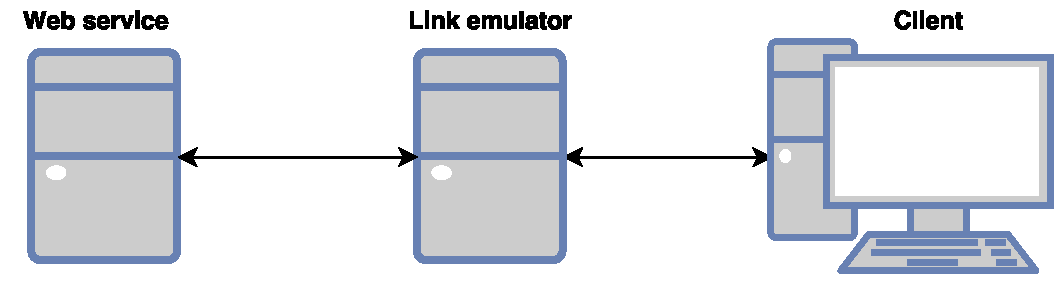
\includegraphics[width=\textwidth]{images/testing_environment_simple.pdf}
\caption{Test setup}
\label{figure-testing-environment-simple}
\end{figure}

\subsection{Linux Network Traffic Control}

The Linux kernel offers a rich set of tools for managing and manipulating the
transmission of packets, referred to as network traffic control. The central
concept in traffic controlling is the concept of queues, which collects entering
packets and dequeues them as fast as the network hardware can accept them.
\textbf{tc} (traffic control) is a Linux program to configure and control the
Linux kernels network scheduler. The \gls{netem} is an enhancement of the
traffic control facilities that allows us to control delay, packet loss and
other characteristics of packets outgoing from a selected network interface
\cite{man-netem}. These tools together enable us to emulate the networks listed
in \cref{table-network-types}.

How to configure \gls{netem} and the Linux traffic control tools is outlined in
the following paragraphs.

\subsubsection{Emulating Network Delays}

With NetEm, we can emulate delays on outgoing packets on a specific link. In
\cref{listing-netem-delay}, we show an example configuration where a fixed delay
of 100 ms to all packets going out of local Ethernet connection.

\begin{lstlisting}[frame=single, language=json, caption="Emulating the delay of outgoing packets", label=listing-netem-delay]
  tc qdisc add dev eth0 parent 1:1 handle 10: \
    netem delay 100ms
\end{lstlisting}

\subsubsection{Emulating the Data Rate}

To emulate different data rates, we use a part of the Linux traffic control tool
called \gls{tbf}. TBF can be used to shape network traffic and ensures that the
configured rate is not exceeded. It shapes traffic based on the concept of
\textit{tokens} and \textit{buckets}. Tokens are generated at the desired data
rate and are collected into buckets, which have a maximum number of tokens they
can store. When TBF receives a packet, it checks if it has a sufficient number
of tokens to send the packet. If not, it is deferred, thus causing an artificial
delay for the packet.

\Cref{listing-netem-data-rate} shows an example configuration where we configure
the maximum data rate of 50 kilobits per second. The burst value is the size of
the bucket in bytes and describes the maximum amount of bytes that tokens can be
available for instantaneously. The limit is the number of bytes that can be
queued waiting for available tokens.

\begin{lstlisting}[frame=single, language=json, caption="Emulating the data rate", label=listing-netem-data-rate]
  tc qdisc add dev eth0 handle 1: \
    root tbf rate 50kbit burst 15000 limit 15000
\end{lstlisting}

\subsubsection{Emulating the Corruption Rate}

The corruption rate allows us to insert random data into a chosen percent of
packets. In \cref{listing-netem-error-rate}, we show how the corruption rate can
be set to 20 percent.

\begin{lstlisting}[frame=single, language=json, caption="Emulating the corruption rate", label=listing-netem-error-rate]
  tc qdisc add dev eth0 parent 1:1 handle 10: \
    netem delay 100ms corrupt 20%
\end{lstlisting}


\subsection{iPerf 3}

iPerf 3 is a tool for measurement of maximum achievable date rate on a network
\cite{iperf3-homepage}. Since we in this thesis are \textit{emulating} different
DIL networks, it is critical that the emulation is as correct and realistic as
possible. Misconfiguration or wrongful emulation could cause us to draw invalid
conclusions. IPerf was one of the recommended tools in a previous study which
explored different network monitoring tools for use in limited capacity
networks \cite{bloebaum-monitoring}.

To confirm and validate our network emulations we use iPerf 3 alongside the
Linux tool \textit{ping}. The measurements are performed between the machine
hosting the client and the machine hosting the Web service. They are performed
before starting the test cases so that the network traffic it generates do not
interfere.


\subsection{Wireshark}

Wireshark is a packet analyzer and allows for performing network usage analysis
\cite{wireshark-homepage}. As an example, this tool allows a user to see all IP
packets sent from a machine over the Ethernet interface.

When performing the testing, we use Wireshark to monitor the network traffic on
the machine hosting the client and its proxy. This is called a packet capture
and allows us to investigate the behavior of the evaluated protocols in the
different types of networks. In particular, we use it to see how many packets
that are sent, as well as the total number of bytes that are sent over the
network.


\section{Test Sets}

For each test network, we perform tests with both a W3C Web service test case
and a RESTful Web service test case. Each test set consists of a Java client and
a Web service. Information about the source code of the test applications is
included in \cref{appendix-source-code} of the appendix.

In this thesis, we look into ways of improving the performance of Web services.
The purpose of the test sets is to imitate network traffic generated by real Web
services. From evaluating the performance increase or decrease of the test
services when using the proxies, we can deduce that this applies to applications
in actual use as well. As performance indicators, we use the average \gls{rtt} as
perceived by the client application and how the network is utilized.

\subsection{NFFI W3C Web Service}

For the purpose of testing W3C Web service applications, we created a mock
system which allows a client to request a service to report positions of
friendly forces. The position report uses the \gls{nffi} format, which has an
associated XML schema with it. We refer to this test case as the "NFFI" test
case.

One test run is illustrated in \cref{figure-nffi-flow} and consists of a client
making a HTTP POST request to the Web service. Associated with the request is an
XML payload which tells the Web service which operation to invoke. In our case,
the service then returns an XML message containing a large number of positions
in the NFFI format.

\begin{figure}[h]
\centering
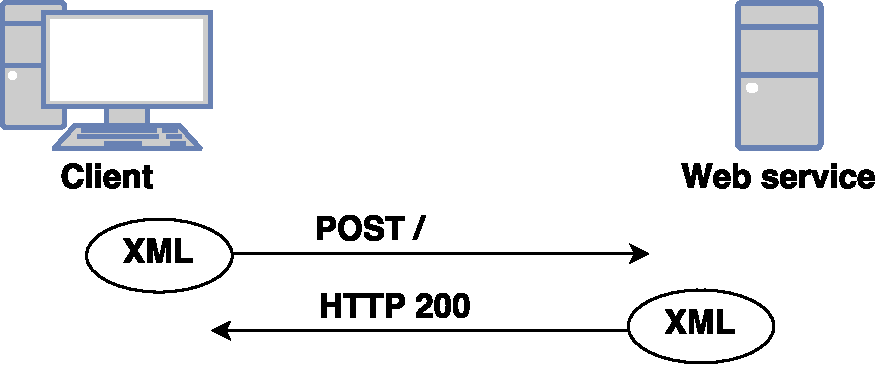
\includegraphics[scale=0.6]{images/nffi_flow.pdf}
\caption{NFFI Web service}
\label{figure-nffi-flow}
\end{figure}

\begin{table}[h]
\begin{tabular}{|l|l|l|l|}
\hline
\textbf{Request URI} & \textbf{HTTP Method} & \textbf{Bytes sent} & \textbf{Bytes received} \\ \hline
?wsdl                & GET                  & 192                 & 3527           \\ \hline
?wsdl=1              & GET                  & 194                 & 4331           \\ \hline
/                    & POST                 & 829                 & 40631          \\ \hline
\textbf{Total:}       & \textbf{3}                     & \textbf{1215}                & \textbf{48489}          \\ \hline
\end{tabular}
\caption{NFFI Web service HTTP requests}
\end{table}


\subsection{RESTful Car Service}

We originally wanted to use a service resembling a military scenario like the
NFFI service. However, no such applications were easily available for testing at
the time of writing the thesis. For the purpose of testing RESTful services, we
chose to develop a small example service ourselves. The RESTful Car service is a
service keeping order of cars in a car registry. It is a simple system keeping
track of the registration number and type description of multiple cars. We refer
to this test case as the "Car system" test case.

 The service exposes an \gls{api} which offers different actions to manage the
 car system. Clients can invoke these operations by using HTTP requests and
 utilizing the associated HTTP method to indicate what to do with a resource.
 Since RESTful services are payload agnostic, we chose \gls{json} to represent
 the data being sent between the server and the client. An example of usage of
 the Car system is illustrated in \cref{figure-rest-flow}.

\begin{figure}[h]
\centering
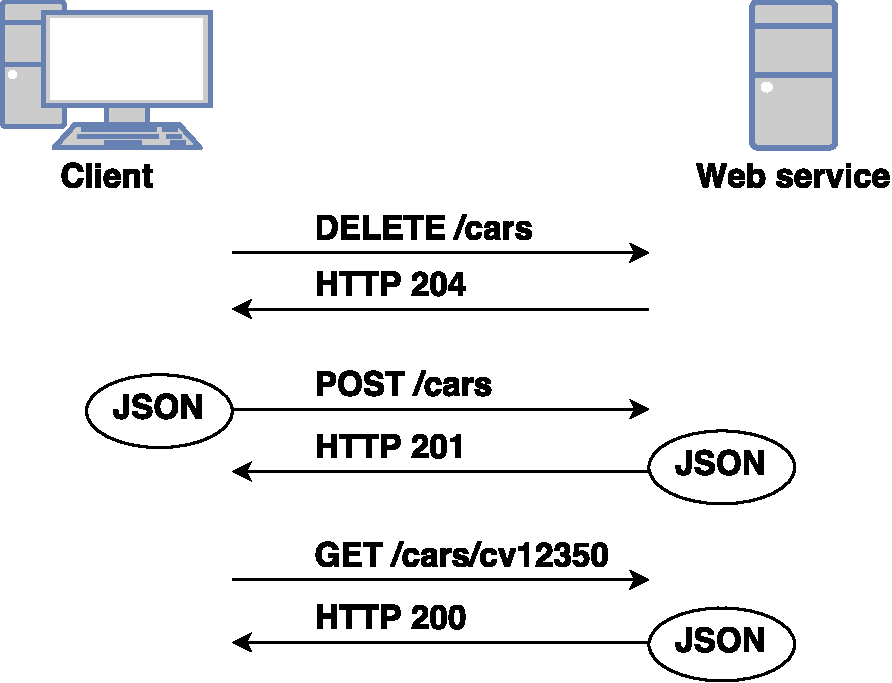
\includegraphics[scale=0.6]{images/rest_flow.pdf}
\caption{Example usage of the REST Car system}
\label{figure-rest-flow}
\end{figure}

Each test run of the Car system consists of a client sequentially invoking the
server with different API requests, listed in \cref{table:car-requests}. The
most common HTTP-methods GET, PUT, POST, and DELETE are all part of the tests.
To test that custom HTTP headers are retained when the HTTP messages are
forwarded through the proxy, both the client and service set a custom header.
When a request or response is received, the application validates that the
custom header is present.



\begin{table}[h]
\begin{tabular}{|l|l|l|l|}
\hline
\textbf{Request URI} & \textbf{HTTP Method} & \textbf{Bytes sent} & \textbf{Bytes received} \\ \hline
/cars                   & DELETE                  & 233                 & 243           \\ \hline
/cars                   & POST                  & 293                 & 353           \\ \hline
/cars                    & POST                 & 298                 & 358           \\ \hline
/cars                    & POST                 & 294                 & 354           \\ \hline
/cars                    & POST                 & 299                 & 359           \\ \hline
/cars                    & POST                 & 296                 & 356           \\ \hline
/cars                    & GET                 & 198                 & 538           \\ \hline
/cars/{id}                    & GET                 & 209                 & 348           \\ \hline
/cars/{id}                    & PUT                 & 309                 & 243           \\ \hline
/cars/{id}                   & GET                 & 209                 & 354           \\ \hline
/cars/{id}                   & DELETE                 & 244                 & 243           \\ \hline
/cars/                   & GET                 & 198                 & 495           \\ \hline
\textbf{Total:}       & \textbf{12}               & \textbf{3080}                & \textbf{4244}          \\ \hline
\end{tabular}
\caption{REST Car system HTTP requests}
\label{table:car-requests}
\end{table}


\subsection{Test Applications Summary}

A test run of both the NFFI test case and the Car system test case consists of
sequentially sending HTTP requests to their respective Web service. However,
they have some fundamental differences. The Car system test involves running 12
HTTP requests while the NFFI request only invokes three. Also, the payload of
each request and response is generally much smaller for the Car system tests.
Moreover, the response message of the third request of the NFFI service is
significantly larger than any other request or response.


\section{Test Setup}
\label{testing-environment}

Both test sets consist of one client and one Web service, where the client would
request the service for some sort of action. The client is running on one
computer while the Web service is deployed in the Glassfish 4 application
server on another computer. The specifications of the machines used in the
testing are listed in \cref{table-machines}.

\begin{table}[h]
\begin{tabularx}{\textwidth}{| X | X | X | X |}
\hline
  \textbf{Machine} & \textbf{Client machine} & \textbf{Web service machine} & \textbf{Link emulator}\\ \hline
  Model & Asus UX 31A Notebook & HP EliteBook 6930p & HP Compaq Elite 8000 \\ \hline
  OS & Debian 8.2 & Ubuntu 14.04 & Ubuntu 14.04\\ \hline
  Kernel & 3.16.0-4-amd64 & 3.13.0-79-generic & 3.19.0-25-generic\\ \hline
  CPU & Intel i7 @ 1.90GHz & Intel Duo T95550 & Intel Quad Q9500 @ 2.83GHz \\ \hline
  Cores & 4 & 2 & 4\\ \hline
  Memory & 4 GB & 4 GB & 12 GB\\ \hline
  Network hardware & ASIX AX88772 USB 2.0 & 82567LM Gigabit & 82567LM-3 Gigabit\\ \hline
  Network interface capacity & 100 Mbit/s & 1 Gbit/s & 1 Gbit/s \\ \hline
\end{tabularx}
\caption{Machines involved in the testing}
\label{table-machines}
\end{table}

\subsection{Network Setup}

The client and Web service machines are connected to each other through a third
computer acting as a link emulator. The link emulator machine has two Ethernet
network cards and interconnects the two other machines. This setup can be seen
in \cref{figure-testing-environment}. For the link emulator to forward IP
packets back and forth between the client and server, IP forwarding is enabled
in the kernel.

\begin{figure}[h]
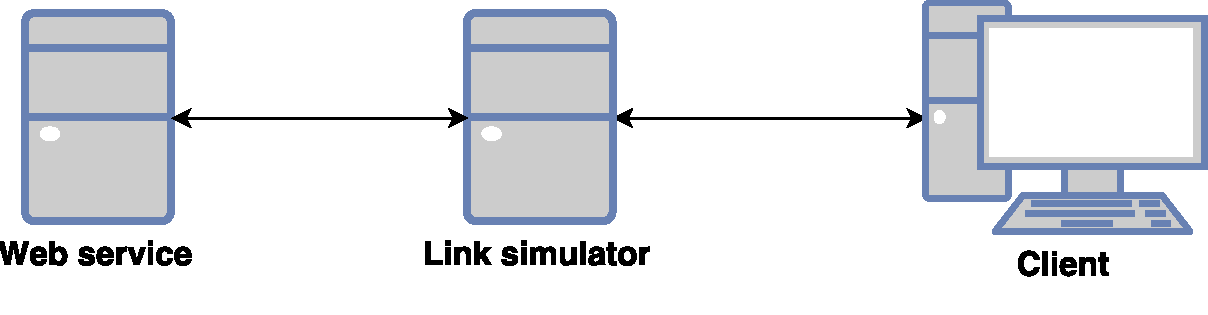
\includegraphics[width=\textwidth]{images/testing_environment.pdf}
\caption{Network used for testing}
\label{figure-testing-environment}
\end{figure}

The client and Web service machine are assigned an IP address in two different
subnets. This is done by the Linux network interface administration program
\textit{ifconfig}. In \cref{listing-ifconfig-client}, the client machine is
assigned the IP address 192.168.11.44.

\begin{lstlisting}[frame=single, language=json, caption="Setting the IP address a network interface", label=listing-ifconfig-client]
ifconfig eth0 192.168.2.1 up
\end{lstlisting}

After setting up the IP addresses, we configure the routing so that the kernel
knows where to route the network traffic. In this case we want all traffic to go
through the link emulator. In \cref{listing-routing} we configure all IP traffic
bound for the subnet 192.168.10.0/24 to be routed through the link emulator with
the IP 192.168.11.1.

\begin{lstlisting}[frame=single, language=json, caption="Configuring routing rules", label=listing-routing]
ip route add unicast 192.168.10.0/24 via 192.168.11.1
\end{lstlisting}

After configuring the IP address and setting up IP routing on both the client
and Web service machine, we start emulating different DIL networks.

\subsubsection{Emulating Different Types of Networks}

Since all network traffic passes through the routing machine, we can control the
flow of IP packets here. As we previously discussed, we make use of the network
traffic control tools of Linux. For each network configuration, a bash script is
run. This script configures the network interface to get the correct network
behavior. Both interfaces are configured so the network is symmetrical in both
directions, except EDGE which has asymmetrical data rates. The bash scripts used
to emulate the DIL networks are included in \cref{appendix-netem-scripts} of the
appendix.


\subsection{Test Execution}

The tests were executed with the setup illustrated in
\cref{figure-testing-setup}. Machine 2 hosts a test client and a proxy, while
machine 1 hosts a proxy and the Web services. The Web services are deployed in a
Glassfish 4 application server. To facilitate AMQP communication between
proxies, a message broker is also run at the Web service machine. In our tests
we use version 5-13.2 of Apache ActiveMQ \cite{activemq-homepage}, an open
source message broker supporting messaging protocols like AMQP and MQTT.

\begin{figure}[h]
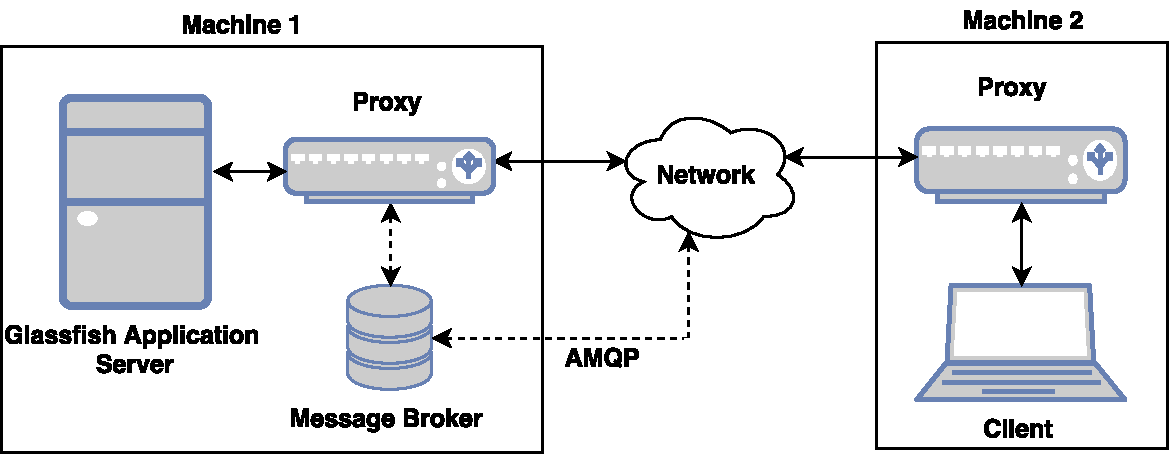
\includegraphics[width=\textwidth]{images/testing_setup.pdf}
\caption{Test setup}
\label{figure-testing-setup}
\end{figure}

Each test execution is initiated from a Java client on machine 2. We then
measure how long it takes to complete all requests part of the test, thus
allowing us to measure the Route Trip Time (RTT) as perceived by the client. All
tests are performed at least 10 times to calculate the mean, standard deviation,
and variance. The results used to create the graphs presented in the following
sections are included in the appendix, \cref{appendix-results}.


Moreover, for each test we perform a packet capture with Wireshark of one sample
test run. The capture allows us to get an indicator of the network usage of the
proxies and the different inter-proxy communication protocols. It is worth
noting that this was only performed on one test case for each test. Thus, any
variance between test runs may not have detected. This is especially true for
the networks with a chance of packet errors. However, it gives us an idea of
the network traffic during that test.

The tests are performed with the following parameters:

\begin{itemize}

    \item Without and with proxies.

    \item GZIP compression on/off. When testing without proxies, the messages
    are \textit{not} compressed.

    \item The protocol used to communicate between the proxies. We refer to
    proxies using HTTP as the inter-proxy communication protocol as a HTTP
    proxy, using AMQP as an AMQP proxy and so on.

\end{itemize}



\section{Function Tests}

The first part of the testing is performed without any intended limitations to
the network. The objective of the function tests is to validate that the proxy
fulfills the functional requirements we sat in chapter 4:

\begin{itemize}
    \item Receive and forward HTTP requests.
    \item Retain HTTP request and response headers.
    \item Support GZIP compression of payload.
    \item Support usage of different transport protocols between the proxies.
\end{itemize}

 In addition, the results from the function tests can be used to benchmark
 against other tests. We run both with and without proxies, allowing us to
 investigate the overhead associated with the usage of proxies. We use the test
 setup described in the last section, although without any intended limitations
 of the network. The tests are performed for both test applications and repeated
 multiple times to get the average \gls{rtt}.

\subsection{Results}

Both the NFFI and Car system test cases finish successfully within the average
of 200 ms when not using proxies. \Cref{figure:results-function-testsx} shows
the results from the function tests and reveals the impact of introducing the
usage of proxies. When using proxies, all test cases still completes
successfully, but their average RTT varies depending on the protocol. The
clients HTTP requests are forwarded through the proxies to the Web service,
which successfully returns a HTTP response back. We also verified that a custom
HTTP header added by the Car system client and Web service are successfully
retained. Together with the successful GZIP compression, the functional
requirements for the proxy is therefore identified as fulfilled.

\subsubsection{Analysis}

Even in an unlimited network, we still see a significant difference between the
protocols. These trends may be the same or perhaps reinforced when the protocols
are used in DIL networks. Therefore, in the coming paragraphs, we investigate
and discuss the possible underlying reasons for the results we obtained in the
function tests.

In test cases without compression, using proxies results in a longer RTT. The
longer RTT can be due to the overhead of sending requests through proxies, which
includes initializing TCP connections and the time the proxies use processing
requests. When using a HTTP proxy with compression, we see a decrease in the RTT
for the NFFI test case. Inspecting the network traffic with Wireshark reveals
the probable cause for this. Compressing the relatively large XML documents sent
in NFFI test case yield a very high compression rate. The compression rates of
the rather small JSON documents in the Car System test case are relatively small
in comparison.

Furthermore, we observe that the transport protocol used by the proxies has a
significant impact on the RTT and packets sent over the network.
\Cref{table:function-test-packets-nffi} and
\cref{table:function-test-packets-rest} list the IP packets sent over the
networks of one sample run of the two test cases. To better understand the
reasons for the difference in average RTT and network usage, we are in the
following sections investigating the behavior of each protocol separately.

\subsubsection{HTTP Proxy}

The HTTP proxy generally performed well. For the NFFI test case with
compression, the proxy is marginally faster than when not using a proxy. The
reduction of data sent and received over the network is reflected by the reduced
number of IP packets. Without compression and for the Car system test case, the
RTT of the HTTP proxy is marginally longer. The reason could be the overhead
associated with the proxy. Using Wireshark we analyzed one sample run of the Car
system test using a HTTP proxy and found the following network activities:

\begin{enumerate}

    \item The Car system client starts invoking its first HTTP request. This is
    a DELETE request without a message body. Since requests are proxied through
    the HTTP proxy, a TCP connection between the client application and the
    proxy is established.

    \item After receiving the request from the client, the proxy establishes a
    TCP connection with the other proxy.

    \item The HTTP request is sent from the proxy to the other proxy. The DELETE
    request has now been converted to a POST request, and the message body
    contains the proxy message. Since the request now has a message body, two
    HTTP headers have been appended: Content-Type and Content-Length. Besides,
    the HTTP-header breadcrumbID has been added, a header used by Camel.
    Including the proxy message, the size of the original HTTP request has now
    grown from 243 to 635 bytes.

	\item A HTTP response is returned from the other proxy. It consists of two
	reassembled TCP segments with the total size of 974  bytes. Comparing with the
	response from when not using a proxy, indicates a few things. Without the
	proxy, the response to the DELETE request is without a message body, while
	with, the HTTP body contains a proxy message. In addition, the response has
	additional HTTP headers than the original request. For this examined response,
	using the proxy introduced a message overhead of 756 bytes.

    \item The response if forwarded from the proxy to the client.

    \item The client starts its next request and repeats the mentioned steps.
    However, since the TCP connections now are initialized and open, both
    between the client and proxy and between the proxies, the TCP connections
    are reused.


  \end{enumerate}

Using a HTTP proxy successfully forwarded messages, but introduced some
overhead. HTTP headers are added and possibly duplicated, as the proxy
encapsulates the original headers inside the proxy message and then adds
its own headers to the HTTP request between the proxies.


\subsubsection{AMQP Proxy}

AMQP had the worst average RTT of the proxy protocols, especially for the Car
system test case. As seen in \cref{table:function-test-packets-nffi} and
\cref{table:function-test-packets-rest}, AMQP sends a lot more IP packets
through the network than HTTP. Since AMQP is broker based, communication occurs
through a message broker and not directly between the proxies. Using Wireshark,
we dived down into the details:

\begin{enumerate}

	\item A TCP connection between the test client and  proxy is first established.

    \item The proxy establishes a TCP connection with the message broker.

    \item The proxy and message broker agree on an AMQP version by exchanging
    the AMQP protocol header.

	 \item Next, to forward the first request, the proxy initiates an AMQP
	 connection. The connection initialization consists of numerous AMQP frames
	 being sent between the proxy and message broker. It includes sending the
	 AMQP frames Open, Begin, Attach and Flow.  First after sending these frames,
	 the first \textit{transfer} frame carrying the message is sent.

     \item Finally, when a response is returned, both the AMQP and TCP connection
     between the proxy and message broker are closed.

     \item The proxy returns the response back to the test client.

     \item When the next test HTTP request is initiated by the client, these
     steps are repeated.

\end{enumerate}

Although all requests are successfully forwarded, the AMQP proxy cause a
significant overhead due to its complex connection procedures. For every request
that is forwarded through the proxy, a new AMQP and TCP connection had to be
established.

\subsubsection{CoAP Proxy}

Using CoAP as the inter-proxy communication protocol had roughly the same
average RTT as the HTTP proxy, with one exception. In the uncompressed NFFI test
case, it had a longer RTT and sent an unreasonable higher amount of packets. We
discuss the possible reasons for this in detail in
\cref{section:evaluation-discussion}. For the test cases not involving large
messages, however, CoAP sent significantly \textit{fewer} IP packets than the
other proxy protocols. Using Wireshark we looked into the network traffic of the
Car system test:

\begin{enumerate}

    \item The test client first establishes a TCP connection with the proxy and sends
    the first message.

    \item The proxy forwards the request in a UDP message to the other proxy.

    \item The other proxy returns the response and acknowledgment in one UDP
    message.

    \item The proxy returns the response to the test client.

    \item The test client invokes a new request, and the steps are repeated.


\end{enumerate}

As we see, CoAP has a more simple messaging pattern compared to AMQP and partly
also HTTP/TCP. CoAP uses UDP, which is a connection-less protocol, which means
that no packets have to be sent to establish a connection. For the
function tests, we see that the CoAP proxy is the proxy with the least network
footprint.

The function tests were done in an unlimited network, so our findings are not
necessarily applicable to DIL networks. In \cref{section:tests-limited}, we put
the proxy and protocols to the test in more limited networks. However, first, in
the next section we see how the proxies cope with the disconnect and
intermittent aspect of the DIL.


\begin{landscape}
    \begin{figure}
    \centering
    \begin{floatrow}
        \ffigbox[\FBwidth]
    {
    \subfloat[NFFI]{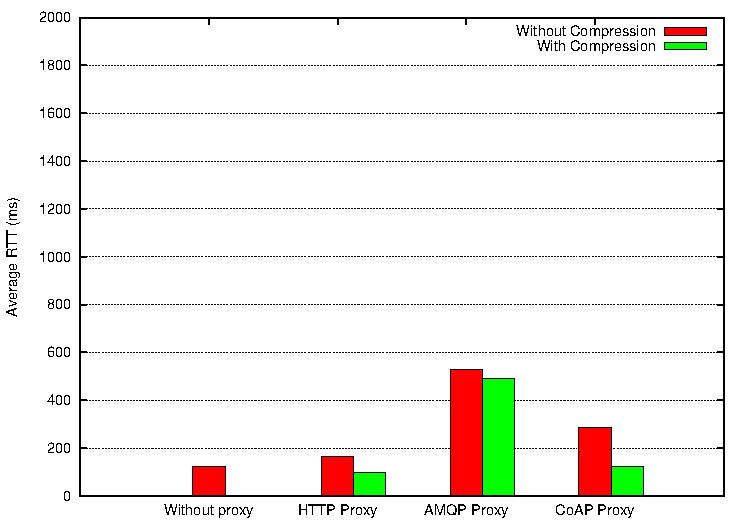
\includegraphics[width=0.5\textwidth]{../results/function_tests/nffi/output/result.pdf}}
    \subfloat[REST]{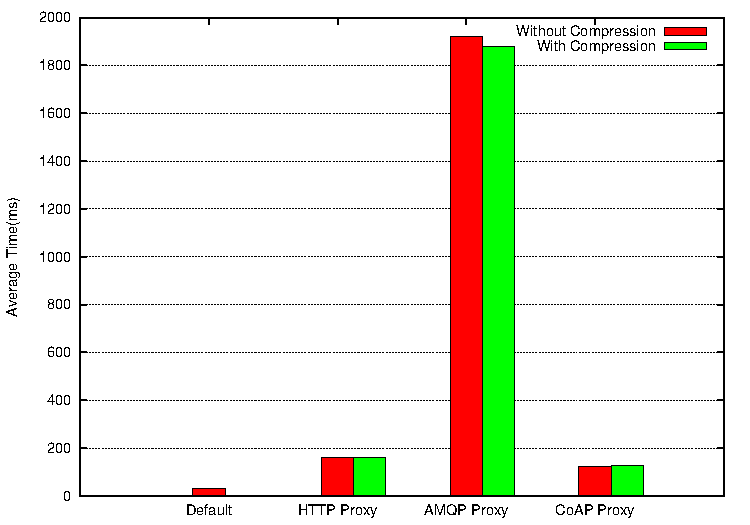
\includegraphics[width=0.5\textwidth]{../results/function_tests/rest/result.pdf}}
    }
    {
    \caption{Function tests - Average RTT Time for the client application.}
    \label{figure:results-function-testsx}
    }
    \end{floatrow}

    \end{figure}
\end{landscape}


\begin{table}[h]
\begin{tabular}{|l|l|l|}
\hline
\textbf{Test} & \textbf{Packets sent} & \textbf{Packets received} \\ \hline
Without Proxy                    &51         & 46        \\ \hline 
Proxy with HTTP                  &45         & 44        \\ \hline 
Proxy with HTTP \& GZIP          &13         & 13        \\ \hline 
Proxy with AMQP                  &73         & 94        \\ \hline 
Proxy with AMQP \& GZIP          &57         & 62        \\ \hline 
Proxy with CoAP                  &101        & 101       \\ \hline 
Proxy with CoAP \& GZIP          &11         & 11        \\ \hline 
\end{tabular}
\caption{NFFI Function test - IP Packets sent and received by the client application.}
\label{table:function-test-packets-nffi}
\end{table}

\begin{table}[h]
\begin{tabular}{|l|l|l|}
\hline
\textbf{Test} & \textbf{Packets sent} & \textbf{Packets received} \\ \hline
Without Proxy                    &25         & 21        \\ \hline 
Proxy with HTTP                  &28         & 26        \\ \hline 
Proxy with HTTP \& GZIP          &28         & 28        \\ \hline 
Proxy with AMQP                  &180        & 203       \\ \hline 
Proxy with AMQP \& GZIP          &190        & 207       \\ \hline 
Proxy with CoAP                  &12         & 12        \\ \hline 
Proxy with CoAP \& GZIP          &12         & 12        \\ \hline 
\end{tabular}
\caption{REST Function test - IP Packets sent and received by the client application.}
\label{table:function-test-packets-rest}
\end{table}




\section{DIL Tests - Intermittent and Disconnected}

\textit{Intermittent} and \textit{disconnected} refers to the network connection
being lost for some period, but then regained again. Disconnected refers to the loss
of connection over a longer period, while intermittent is a special case of
disconnected and refers to shorter disruptions. The requirements we set for our
proxy were that it should:

\begin{itemize}

    \item Handle frequent network disruptions.
    \item Handle disconnects over longer periods of time.

\end{itemize}



In our testing, we focus on the loss of connections for longer periods of time.
The objective of this testing is to evaluate how the proxy manages disconnects.
We define the success criteria to be that a client can eventually process his
request after the connection is reestablished. The client's HTTP request should
not be interrupted in any way, other than it taking a longer time to process the
request.

\subsection{Execution}

 The tests are performed over an unlimited network and for both the NFFI and Car
 system test. The proxy redelivery delay is configured to be with a fixed
 20-second retransmission. The tests are executed by starting the test
 applications and then immediately removing the Ethernet cable between the
 client machine and the link emulator as illustrated in
 \cref{figure-testing-disconncted}. We then wait around 60 seconds, allowing
 requests to trigger timeouts and thus invoking the proxy redelivery mechanism.
 Finally, we connect the cable again and observe if the test application is able
 to finish its requests successfully.

 \begin{figure}[h]
 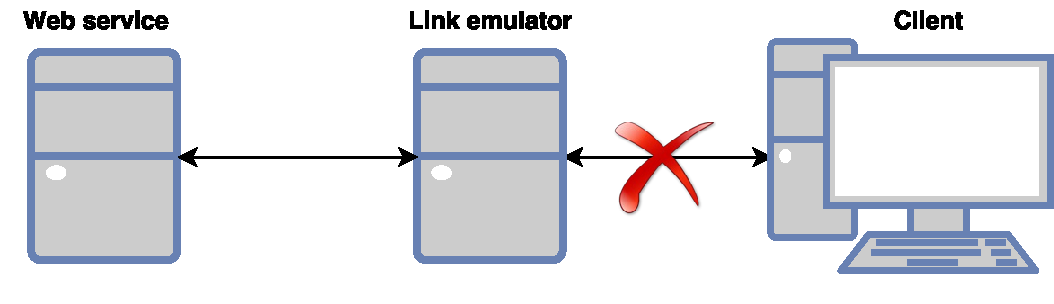
\includegraphics[width=\textwidth]{images/testing_disconnected.pdf}
 \caption{Emulating a disconnect}
 \label{figure-testing-disconncted}
 \end{figure}


\subsection{Results and Analysis}

For both the REST and W3C Web service test scenarios, the results were
identical. Without using proxies, the connection timed out, and the applications
were unable to continue as shown in \cref{table:disconnected-nffi} and
\cref{table:disconnected-rest}. With proxies, the connection did not time out,
and the protocols retransmission mechanisms were able to continue transmission
when the connection was reestablished.


\begin{table}[h!]
\begin{tabular}{| l | l |}
\hline
  \textbf{Test} & \textbf{Result} \\ \hline
  Without proxy & Connection timeout \\ \hline
  Proxy with HTTP & Success \\ \hline
  Proxy with AMQP & Success \\ \hline
  Proxy with CoAP & Success \\ \hline
\end{tabular}
\caption{NFFI Web service results}
\label{table:disconnected-nffi}
\end{table}

\begin{table}[h!]
\begin{tabular}{| l | l |}
\hline
  \textbf{Test} & \textbf{Result} \\ \hline
  Without proxy & Connection timeout \\ \hline
  Proxy with HTTP & Success \\ \hline
  Proxy with AMQP & Success \\ \hline
  Proxy with CoAP & Success \\ \hline
\end{tabular}
\caption{RESTful Web service results}
\label{table:disconnected-rest}
\end{table}


\section{DIL Tests - Limited}
\label{section:tests-limited}

The third DIL characteristic, \textit{limited}, refers to various ways a network
can be constrained. The limited characteristic includes long delays, packet
loss, and low data rate. In this section, we present the testing performed for
the different types of networks identified in \cref{table-network-types}.
Through this testing we evaluate how the proxy performs with regards to
requirement 6, stating that the proxy should be able to:

\begin{itemize}

    \item Handle low data rates, long delays, and high packet error rates.

\end{itemize}



\subsection{Satellite Communication}

In this test network, we emulate \gls{satcom}. With satellite communication, all
data is relayed through a communication satellite in orbit around the earth.
This type of communication is characterized by its low data rate and high delay.

\subsubsection{Results and Analysis}

From the SATCOM testing results presented in \cref{figure:results-satcom},
\cref{table:satcom-test-packets-nffi} and \cref{table:satcom-test-packets-rest},
we observe the following:

\begin{itemize}

    \item The HTTP proxy with compression has the overall best RTT.

    \item With one exception, AMQP has significantly higher RTT than the other
    protocols. For the Car system tests with many subsequent HTTP requests, we
    see that AMQP triggers the sending of many IP packets. In a sample test run,
    the Wireshark capture revealed that AMQP sends twenty times the amount of IP
    packets compared to CoAP.

    \item CoAP struggles with large uncompressed messages of NFFI test case. For
    the Car system test, however, the CoAP proxy has almost equal average RTT as
    the HTTP proxy. A Wireshark capture during the Car system test shows that
    CoAP proxy sends very few of IP packets compared to other protocols.

    \item Compression can be of less importance in networks with high data
    rates and where the long delay is the limiting factor.

\end{itemize}

\begin{landscape}
    \begin{figure}
    \centering
    \begin{floatrow}
        \ffigbox[\FBwidth]
    {
    \subfloat[NFFI]{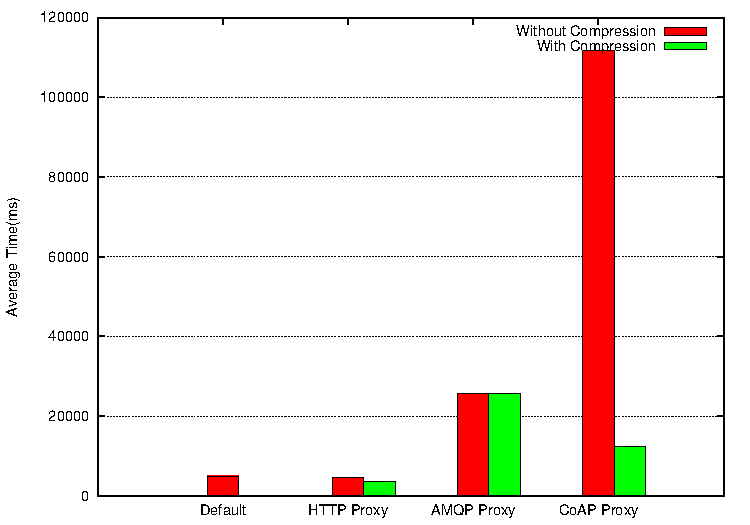
\includegraphics[width=0.5\textwidth]{../results/satellite/nffi/result.pdf}}
    \subfloat[REST]{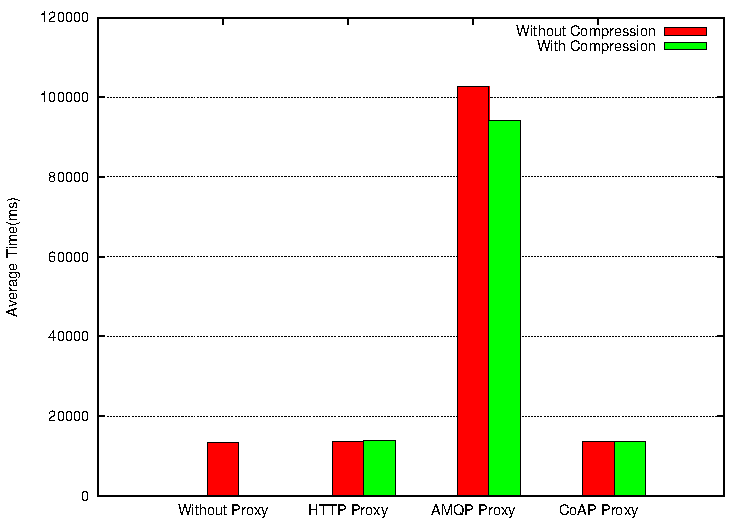
\includegraphics[width=0.5\textwidth]{../results/satellite/rest/result.pdf}}
    }{\caption{SATCOM tests - Average RTT Time for the client application.}
    \label{figure:results-satcom}
    }
    \end{floatrow}
    \end{figure}
\end{landscape}


\begin{table}[h]
\begin{tabular}{|l|l|l|}
\hline
\textbf{Test} & \textbf{Packets sent} & \textbf{Packets received} \\ \hline
Without Proxy                    &54         & 47        \\ \hline 
Proxy with HTTP                  &47         & 45        \\ \hline 
Proxy with HTTP \& GZIP          &16         & 14        \\ \hline 
Proxy with AMQP                  &88         & 102       \\ \hline 
Proxy with AMQP \& GZIP          &71         & 68        \\ \hline 
Proxy with CoAP                  &101        & 101       \\ \hline 
Proxy with CoAP \& GZIP          &11         & 11        \\ \hline 
\end{tabular}
\caption{NFFI SATCOM test - IP Packets sent and received by the client application.}
\label{table:satcom-test-packets-nffi}
\end{table}

\begin{table}[h]
\begin{tabular}{|l|l|l|}
\hline
\textbf{Test} & \textbf{Packets sent} & \textbf{Packets received} \\ \hline
Without Proxy                    &27         & 22        \\ \hline 
Proxy with HTTP                  &26         & 25        \\ \hline 
Proxy with HTTP \& GZIP          &30         & 28        \\ \hline 
Proxy with AMQP                  &244        & 238       \\ \hline 
Proxy with AMQP \& GZIP          &240        & 240       \\ \hline 
Proxy with CoAP                  &12         & 12        \\ \hline 
Proxy with CoAP \& GZIP          &12         & 12        \\ \hline 
\end{tabular}
\caption{REST SATCOM test - IP Packets sent and received by the client application.}
\label{table:satcom-test-packets-rest}
\end{table}




\subsection{Line-of-Sight}

In this test scenario, we emulate \gls{los} networks which are characterized by
being a radio-based type of network with no physical obstacles between the nodes
in the network. LOS has high data rate, low delay, and zero error rate.

\subsubsection{Results and Analysis}

The average RTT of the LOS tests is shown in \cref{los:results-satcom}. IP
packets sent and received in a sample run of the NFFI and Car system test cases
are listed in \cref{table:los-test-packets-nffi} and
\cref{table:los-test-packets-rest}. The significant findings are summarized
here:

\begin{itemize}

    \item HTTP proxy yielded the lowest average RTT in the NFFI test case, while
    not using a proxy had the best RTT in the Car system test. In the Car system
    tests, the CoAP proxy is marginally faster than a HTTP proxy.

    \item We observe the same trends regarding CoAP and AMQP as in the function
    testing. The LOS type of network is a relatively unlimited network. The results
    have the same characteristics as the results from the function tests.

    \item For the Car system test, we see that enabling compression yields a
    slightly longer average RTT. The reason for this can be the time used to
    compress the payload is larger than the time saved by reducing the size of
    the message.

\end{itemize}



\begin{landscape}
    \begin{figure}
    \centering
    \begin{floatrow}
        \ffigbox[\FBwidth]
    {
    \subfloat[NFFI]{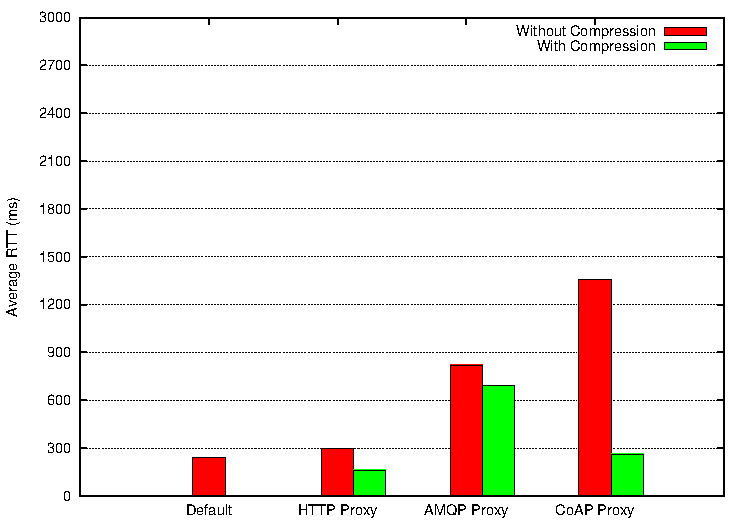
\includegraphics[width=0.5\textwidth]{../results/los/nffi/result.pdf}}
    \subfloat[REST]{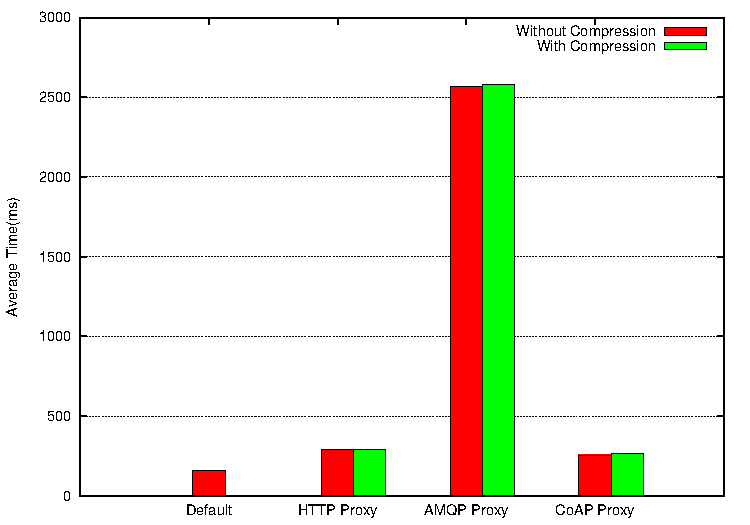
\includegraphics[width=0.5\textwidth]{../results/los/rest/result.pdf}}
    }{\caption{LOS tests - Average RTT Time for the client application.}
        \label{los:results-satcom}
    }
    \end{floatrow}
    \end{figure}
\end{landscape}

\begin{table}[h]
\begin{tabular}{|l|l|l|}
\hline
\textbf{Test} & \textbf{Packets sent} & \textbf{Packets received} \\ \hline
Without Proxy                    &46         & 43        \\ \hline 
Proxy with HTTP                  &43         & 44        \\ \hline 
Proxy with HTTP \& GZIP          &14         & 13        \\ \hline 
Proxy with AMQP                  &68         & 91        \\ \hline 
Proxy with AMQP \& GZIP          &54         & 59        \\ \hline 
Proxy with CoAP                  &101        & 101       \\ \hline 
Proxy with CoAP \& GZIP          &11         & 11        \\ \hline 
\end{tabular}
\caption{NFFI LOS test - IP Packets sent and received by the client application.}
\label{table:los-test-packets-nffi}
\end{table}

\begin{table}[h]
\begin{tabular}{|l|l|l|}
\hline
\textbf{Test} & \textbf{Packets sent} & \textbf{Packets received} \\ \hline
Without Proxy                    &25         & 21        \\ \hline 
Proxy with HTTP                  &28         & 26        \\ \hline 
Proxy with HTTP \& GZIP          &24         & 24        \\ \hline 
Proxy with AMQP                  &189        & 201       \\ \hline 
Proxy with AMQP \& GZIP          &187        & 201       \\ \hline 
Proxy with CoAP                  &12         & 12        \\ \hline 
Proxy with CoAP \& GZIP          &12         & 12        \\ \hline 
\end{tabular}
\caption{REST LOS test - IP Packets sent and received by the client application.}
\label{table:los-test-packets-rest}
\end{table}




\subsection{WiFi 1}

With this type of network, we emulate communication over WiFi where the
conditions are relatively good. The data rate is high, the delay is moderate,
and the packet error rate is 1 \%.

\subsubsection{Results and Analysis}

The results of the tests in this type of network are presented in
\cref{figure:wifi1-results}, \cref{table:wifi1-test-packets-nffi} and
\cref{table:wifi1-test-packets-rest}. We see the following:

\begin{itemize}

    \item Again we observe the same trends from previous tests. AMQP has the
    longest average RTT while CoAP struggle with large messages.

    \item For the NFFI test, HTTP proxy with compression yields the lowest
    average RTT.

    \item For the Car system tests, running without using proxies have the
    lowest average RTT.

\end{itemize}


\begin{landscape}
    \begin{figure}
    \centering
    \begin{floatrow}
        \ffigbox[\FBwidth]
    {
    \subfloat[NFFI]{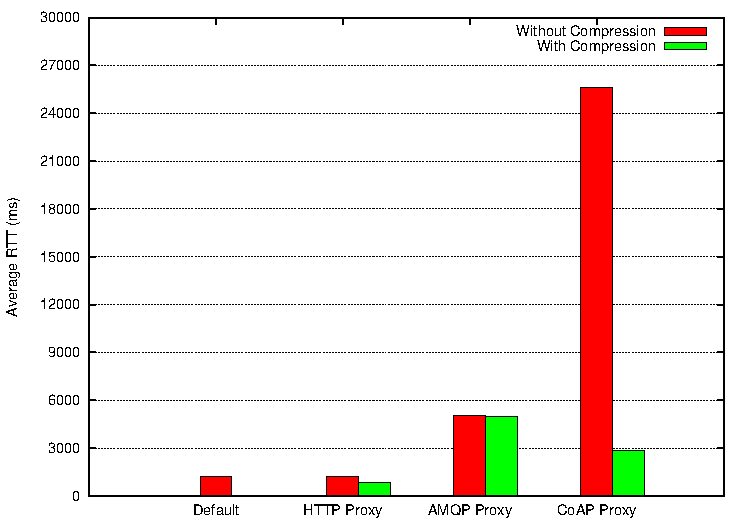
\includegraphics[width=0.5\textwidth]{../results/wifi1/nffi/result.pdf}}
    \subfloat[REST]{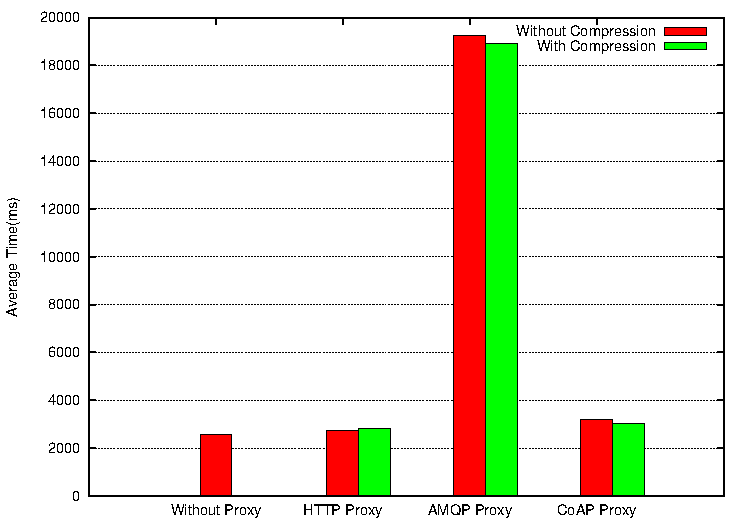
\includegraphics[width=0.5\textwidth]{../results/wifi1/rest/result.pdf}}
    }{\caption{WiFi 1 tests - Average RTT Time for the client application.}
\label{figure:wifi1-results}
    }
    \end{floatrow}
    \end{figure}
\end{landscape}

\begin{table}[h]
\begin{tabular}{|l|l|l|}
\hline
\textbf{Test} & \textbf{Packets sent} & \textbf{Packets received} \\ \hline
Without Proxy                    &50         & 45        \\ \hline 
Proxy with HTTP                  &45         & 45        \\ \hline 
Proxy with HTTP \& GZIP          &13         & 14        \\ \hline 
Proxy with AMQP                  &76         & 93        \\ \hline 
Proxy with AMQP \& GZIP          &60         & 60        \\ \hline 
Proxy with CoAP                  &104        & 104       \\ \hline 
Proxy with CoAP \& GZIP          &22         & 22        \\ \hline 
\end{tabular}
\caption{NFFI WiFi 1 test - IP Packets sent and received by the client application.}
\label{table:wifi1-test-packets-nffi}
\end{table}

\begin{table}[h]
\begin{tabular}{|l|l|l|}
\hline
\textbf{Test} & \textbf{Packets sent} & \textbf{Packets received} \\ \hline
Without Proxy                    &28         & 22        \\ \hline 
Proxy with HTTP                  &26         & 24        \\ \hline 
Proxy with HTTP \& GZIP          &30         & 27        \\ \hline 
Proxy with AMQP                  &192        & 211       \\ \hline 
Proxy with AMQP \& GZIP          &198        & 208       \\ \hline 
Proxy with CoAP                  &12         & 12        \\ \hline 
Proxy with CoAP \& GZIP          &12         & 12        \\ \hline 
\end{tabular}
\caption{REST WiFi 1 test - IP Packets sent and received by the client application.}
\label{table:wifi1-test-packets-rest}
\end{table}


\subsection{WiFi 2}

This type of network also emulates wireless communication, but instead in the
``outer'' areas of the wireless range. It has good data rate, moderate delay,
and very high packet error rate (20 \%).


\subsubsection{Results and Analysis}

\Cref{figure:wifi2-results} shows the average response times of the WiFi 2 test
cases. \Cref{table:wifi2-test-packets-nffi} and
\cref{table:wifi2-test-packets-rest} list the packets sent and received from the
test applications in a sample test run. For the tests ran in an emulated WiFi 2
network, we see the following:

\begin{itemize}

    \item A significantly longer average RTT for all test cases. The variance of
    the test results has increased compared to the other test networks. The high
    variance can be attributed to the high probability of packet errors, since
    some test runs may experience few errors, while other more.

    \item The HTTP proxy with compression had the overall best average
    RTT.

    \item In the NFFI test case with a CoAP proxy without compression, the proxy
    was not able to forward the request. The reason for this is that the CoAP
    request between the proxies timed out. The retransmission mechanism of the
    proxy was invoked, but the consecutive attempts were unsuccessfully as well.
    Furthermore, we observe that even with compression did the CoAP proxy have a longer
    average RTT than the other proxies protocols.

    \item We also see that for the NFFI test cases, compressing the messages
    yields a substantial performance increase with regards to the average RTT.
    This is probably due to since fewer IP packets need to be sent over the
    network, it is a less chance for packet errors.

\end{itemize}


\begin{landscape}
    \begin{figure}
    \centering
    \begin{floatrow}
        \ffigbox[\FBwidth]
    {
    \subfloat[NFFI]{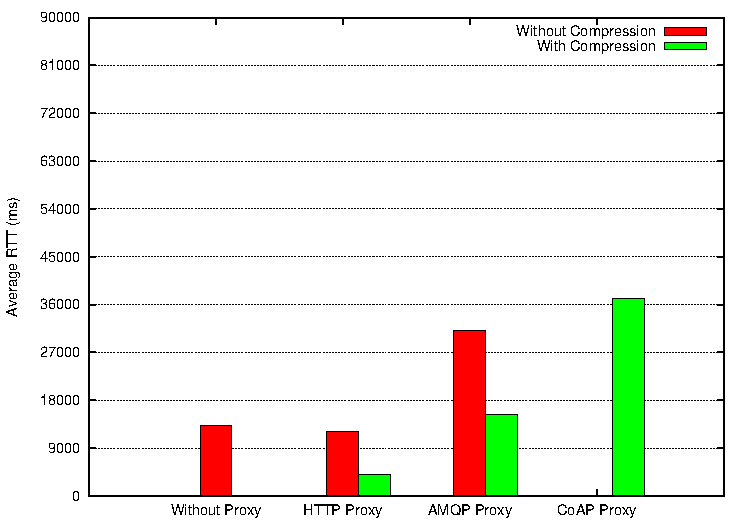
\includegraphics[width=0.5\textwidth]{../results/wifi2/nffi/result.pdf}}
    \subfloat[REST]{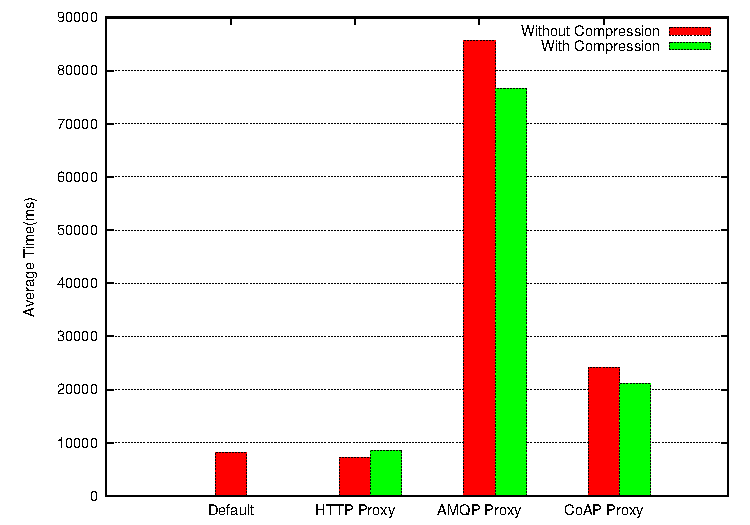
\includegraphics[width=0.5\textwidth]{../results/wifi2/rest/result.pdf}}
    }{\caption{WiFi 2 tests - Average RTT Time for the client application.}
\label{figure:wifi2-results}
    }
    \end{floatrow}
    \end{figure}
\end{landscape}

\begin{table}[h]
\begin{tabular}{|l|l|l|}
\hline
\textbf{Test} & \textbf{Packets sent} & \textbf{Packets received} \\ \hline
Without Proxy                    &51         & 54        \\ \hline 
Proxy with HTTP                  &45         & 52        \\ \hline 
Proxy with HTTP \& GZIP          &15         & 13        \\ \hline 
Proxy with AMQP                  &101        & 111       \\ \hline 
Proxy with AMQP \& GZIP          &76         & 71        \\ \hline 
Proxy with CoAP                  &0          & 0         \\ \hline 
Proxy with CoAP \& GZIP          &14         & 12        \\ \hline 
\end{tabular}
\caption{NFFI WiFi 2 test - IP Packets sent and received by the client application.}
\label{table:wifi2-test-packets-nffi}
\end{table}

\begin{table}[h]
\begin{tabular}{|l|l|l|}
\hline
\textbf{Test} & \textbf{Packets sent} & \textbf{Packets received} \\ \hline
Without Proxy                    &32         & 39        \\ \hline 
Proxy with HTTP                  &37         & 30        \\ \hline 
Proxy with HTTP \& GZIP          &31         & 28        \\ \hline 
Proxy with AMQP                  &332        & 317       \\ \hline 
Proxy with AMQP \& GZIP          &231        & 243       \\ \hline 
Proxy with CoAP                  &18         & 15        \\ \hline 
Proxy with CoAP \& GZIP          &24         & 17        \\ \hline 
\end{tabular}
\caption{REST WiFi 2 test - IP Packets sent and received by the client application.}
\label{table:wifi2-test-packets-rest}
\end{table}

\subsection{Combat Net Radio}

\gls{cnr} is characterized by its very low data rate, moderate timeout and packet
error rate of 1 \%.


\subsubsection{Results and Analysis}

In \cref{figure:cnr-results} we show the average RTT of the tests for the
emulated \gls{cnr} network. \Cref{table:cnr-test-packets-nffi}
\cref{table:cnr-test-packets-rest} shows the IP packets sent/received in a sample
run of the test cases. We observe the following:

\begin{itemize}

    \item CoAP proxy with compression had the best average RTT and sent the
    fewest number of IP packets.

    \item The NFFI tests without compression have a very high average RTT.

    \item The AMQP test without compression was not able to
    complete before it timed out.

    \item If we compare the test cases without proxy and proxy with HTTP, we can
    see the overhead caused by using proxies. The increased HTTP message size
    caused by the proxy leads to a higher average RTT.

\end{itemize}

\begin{landscape}
    \begin{figure}
    \centering
    \begin{floatrow}
        \ffigbox[\FBwidth]
    {
    \subfloat[NFFI]{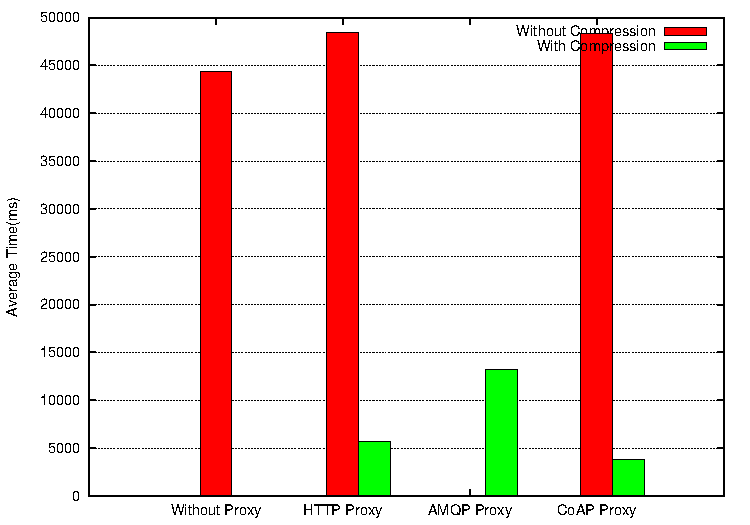
\includegraphics[width=0.5\textwidth]{../results/cnr/nffi/result.pdf}}
    \subfloat[REST]{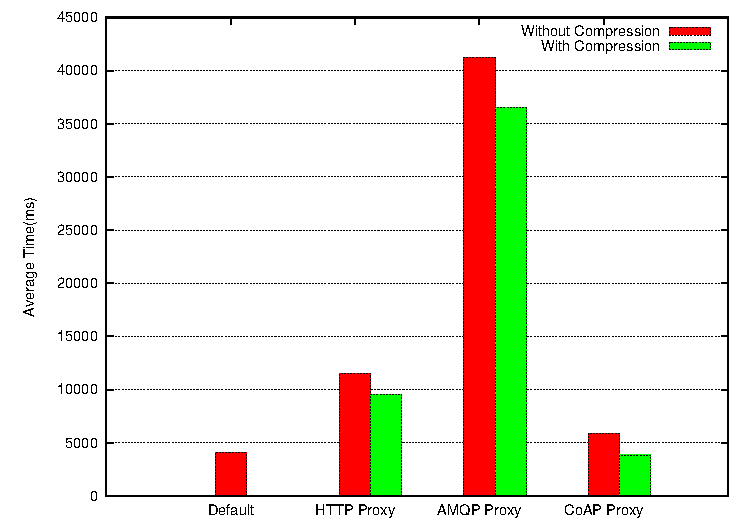
\includegraphics[width=0.5\textwidth]{../results/cnr/rest/result.pdf}}
    }{\caption{CNR tests - Average RTT Time for the client application.}
        \label{figure:cnr-results}
    }
    \end{floatrow}
    \end{figure}
\end{landscape}

\begin{table}[h]
\begin{tabular}{|l|l|l|}
\hline
\textbf{Test} & \textbf{Packets sent} & \textbf{Packets received} \\ \hline
Without Proxy                    &70         & 71        \\ \hline 
Proxy with HTTP                  &66         & 67        \\ \hline 
Proxy with HTTP \& GZIP          &14         & 13        \\ \hline 
Proxy with AMQP                  &0          & 0         \\ \hline 
Proxy with AMQP \& GZIP          &56         & 62        \\ \hline 
Proxy with CoAP                  &103        & 103       \\ \hline 
Proxy with CoAP \& GZIP          &11         & 11        \\ \hline 
\end{tabular}
\caption{NFFI CNR test - IP Packets sent and received by the client application.}
\label{table:cnr-test-packets-nffi}
\end{table}

\begin{table}[h]
\begin{tabular}{|l|l|l|}
\hline
\textbf{Test} & \textbf{Packets sent} & \textbf{Packets received} \\ \hline
Without Proxy                    &25         & 21        \\ \hline 
Proxy with HTTP                  &28         & 27        \\ \hline 
Proxy with HTTP \& GZIP          &24         & 24        \\ \hline 
Proxy with AMQP                  &233        & 240       \\ \hline 
Proxy with AMQP \& GZIP          &220        & 225       \\ \hline 
Proxy with CoAP                  &14         & 13        \\ \hline 
Proxy with CoAP \& GZIP          &12         & 12        \\ \hline 
\end{tabular}
\caption{REST CNR test - IP Packets sent and received by the client application.}
\label{table:cnr-test-packets-rest}
\end{table}


\subsection{EDGE}

\gls{edge} is characterized by a low upload data rate and a moderately low
download rate. We emulate EDGE with a moderate delay and zero packet loss.

\subsubsection{Results and Analysis}

\Cref{figure:edge-results} shows the average response times of the EDGE test
cases. \Cref{table:edge-test-packets-nffi} and
\cref{table:edge-test-packets-rest} list the packets sent and received from the
test applications in a sample test run. We observe the following:

\begin{itemize}

    \item HTTP proxy with compression has the overall lowest average RTT.

    \item Again we see that CoAP struggles with large messages.


\end{itemize}

\begin{landscape}
    \begin{figure}
    \centering
    \begin{floatrow}
        \ffigbox[\FBwidth]
    {
    \subfloat[NFFI]{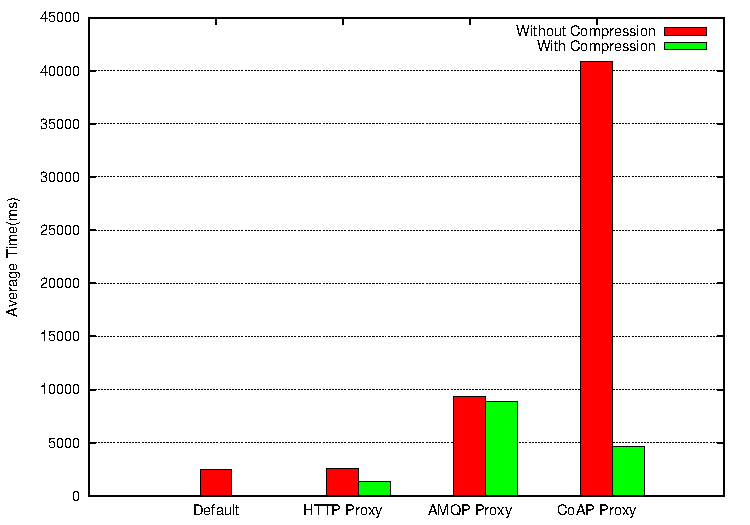
\includegraphics[width=0.5\textwidth]{../results/edge/nffi/result.pdf}}
    \subfloat[REST]{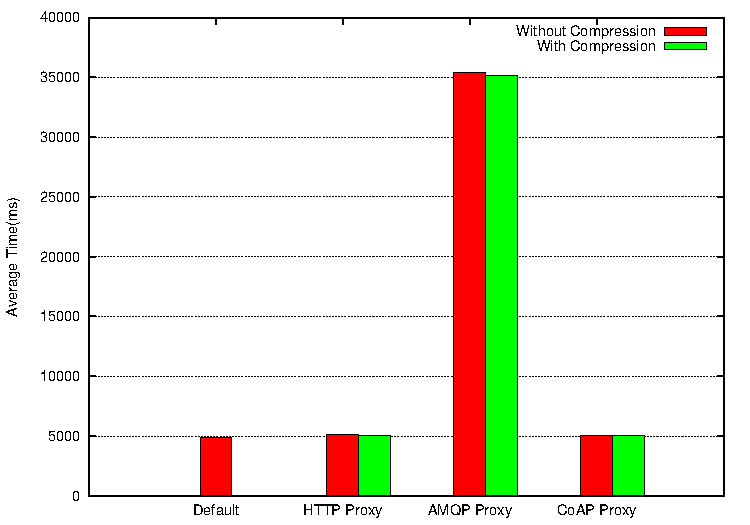
\includegraphics[width=0.5\textwidth]{../results/edge/rest/result.pdf}}
    }{\caption{EDGE tests - Average RTT Time for the client application.}
        \label{figure:edge-results}
    }
    \end{floatrow}
    \end{figure}
\end{landscape}

\begin{table}[h]
\begin{tabular}{|l|l|l|}
\hline
\textbf{Test} & \textbf{Packets sent} & \textbf{Packets received} \\ \hline
Without Proxy                    &50         & 45        \\ \hline 
Proxy with HTTP                  &45         & 44        \\ \hline 
Proxy with HTTP \& GZIP          &14         & 13        \\ \hline 
Proxy with AMQP                  &78         & 95        \\ \hline 
Proxy with AMQP \& GZIP          &59         & 59        \\ \hline 
Proxy with CoAP                  &101        & 101       \\ \hline 
Proxy with CoAP \& GZIP          &11         & 11        \\ \hline 
\end{tabular}
\caption{NFFI CNR test - IP Packets sent and received by the client application.}
\label{table:edge-test-packets-nffi}
\end{table}

\begin{table}[h]
\begin{tabular}{|l|l|l|}
\hline
\textbf{Test} & \textbf{Packets sent} & \textbf{Packets received} \\ \hline
Without Proxy                    &27         & 23        \\ \hline 
Proxy with HTTP                  &28         & 27        \\ \hline 
Proxy with HTTP \& GZIP          &29         & 27        \\ \hline 
Proxy with AMQP                  &194        & 201       \\ \hline 
Proxy with AMQP \& GZIP          &201        & 212       \\ \hline 
Proxy with CoAP                  &12         & 12        \\ \hline 
Proxy with CoAP \& GZIP          &12         & 12        \\ \hline 
\end{tabular}
\caption{REST EDGE test - IP Packets sent and received by the client application.}
\label{table:edge-test-packets-rest}
\end{table}

\section{Experiments with Tactical Broadband}
\label{section:evaluation-kongsberg}


The majority of the testing was performed over software emulated networks. To
validate these results, we performed experiments with military communication
equipment. We used two WM600 radios developed by \gls{kda}, intended for users
"on-the-move". WM600 can be used as IP radios through the Ethernet interface and
support data rates up to 2500 kbit/s \cite{kongsberg-wm600}. A picture of the
radio can be seen in \cref{figure-kdawm600}.

\begin{figure}[h]
\centering
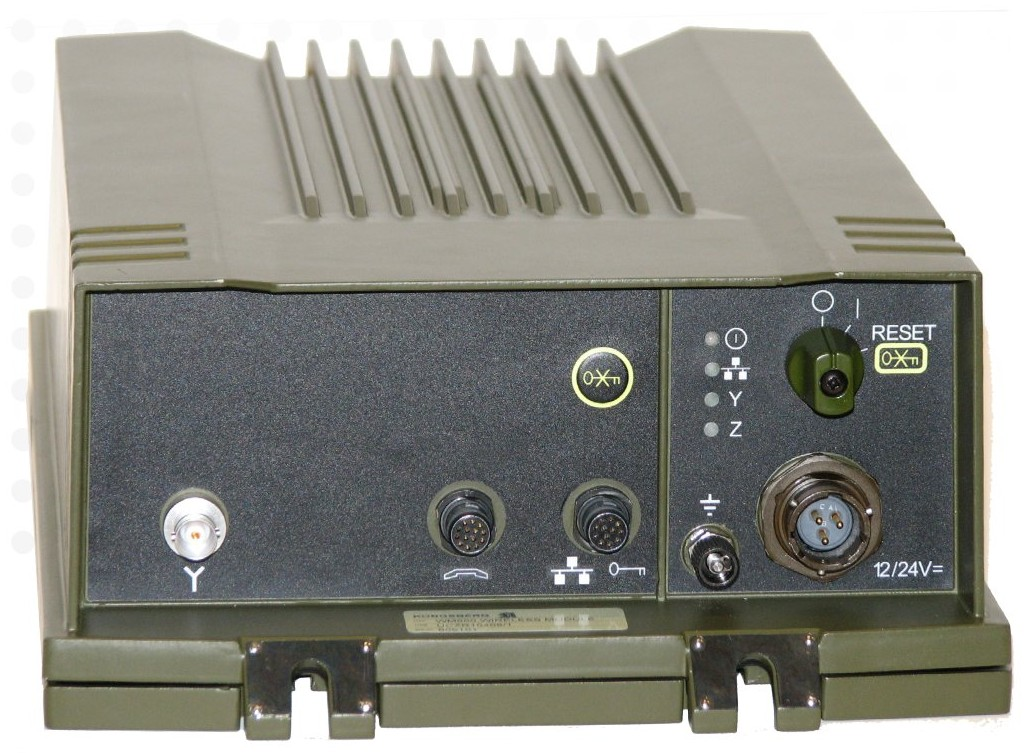
\includegraphics[scale=0.2]{images/kda_wm600.jpg}
\caption{The KDA WM600 radio (from \cite{kongsberg-wm600})}
\label{figure-kdawm600}
\end{figure}

We performed the testing in a communication laboratory located at \gls{ffi} with
the setup illustrated in \cref{figure-radio-testing-environment}. It is a
point-to-point setup with two radios and without any multi-hop functionality.
The radios have the capacity to work as a multi-hop \gls{manet}, but this was not
tested in this thesis. The radios were attached to configurable attenuators,
which could reduce the power of a signal by distorting its waveform. The purpose
of the attenuators is to facilitate radio experiments with varying signal
strength.

During our experiments, the attenuators were set to 30 DB. The measured data
rate of the network was around 90 kbit/s and with a ping response time of 23 ms.

\begin{figure}[h]
\centering
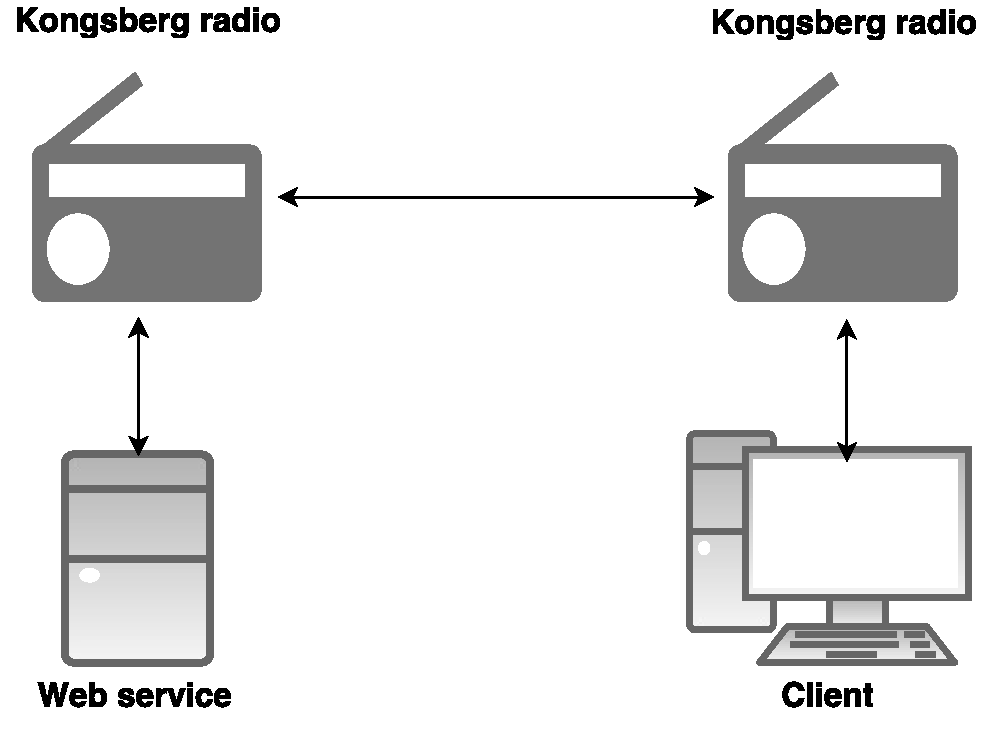
\includegraphics[scale=0.6]{images/radio_testing_environment.pdf}
\caption{Tactical broadband testing environment}
\label{figure-radio-testing-environment}
\end{figure}

\subsubsection{Results and analysis}

\Cref{figure:kongsberg-results} shows the average RTT of the test cases
performed over tactical broadband. We make the following observations:

\begin{itemize}

    \item We see the same trends as in the software emulated networks.

    \item Compression yields a significantly lower RTT for the NFFI tests and a
    small decrease for the Car system tests.

    \item The CoAP proxy struggles with large messages but otherwise has the
    overall best RTT.

\end{itemize}

\begin{landscape}
    \begin{figure}
    \centering
    \begin{floatrow}
        \ffigbox[\FBwidth]
    {
    \subfloat[NFFI]{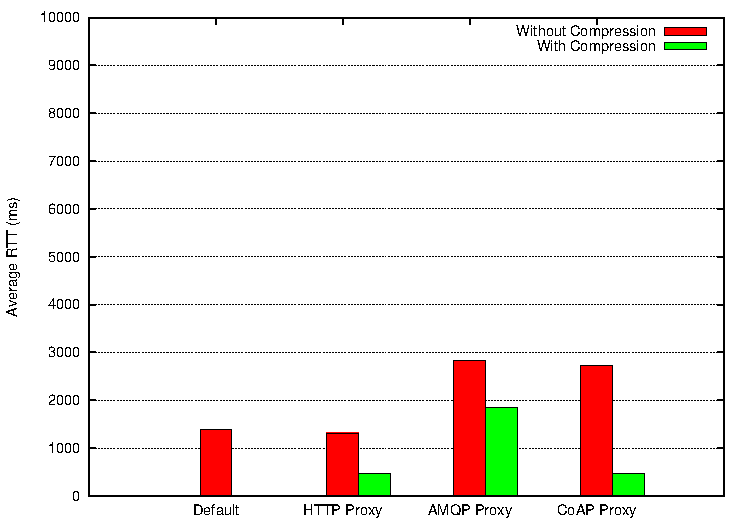
\includegraphics[width=0.5\textwidth]{../results/kongsberg/nffi/result.pdf}}
    \subfloat[REST]{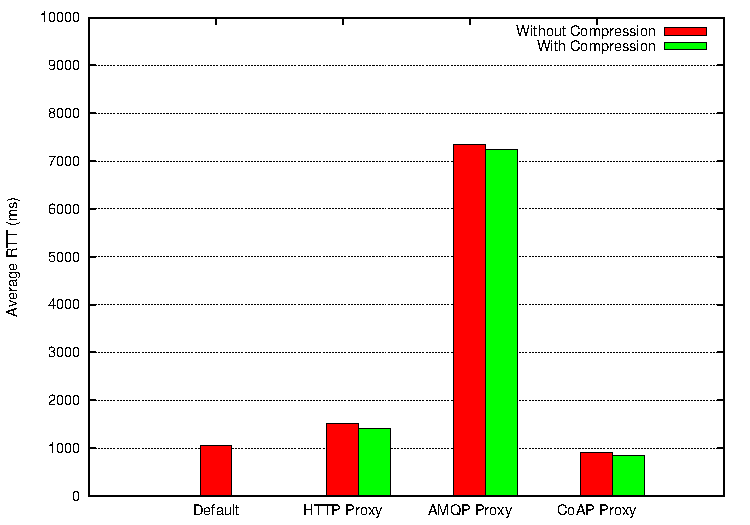
\includegraphics[width=0.5\textwidth]{../results/kongsberg/rest/result.pdf}}
    }{\caption{Tactical Broadband tests - Average RTT Time for the client application.}
        \label{figure:kongsberg-results}
    }
    \end{floatrow}
    \end{figure}
\end{landscape}

\section{Discussion}
\label{section:evaluation-discussion}

In all emulated networks we see some consistent trends. Compressing the messages
between the proxies generally lowered the RTT, especially for large messages of
the NFFI test case. The exception is in some of the DIL networks with relatively
high data rates, the time spent to compress and decompress a message was longer
than the time saved by sending a compressed message.

In all test cases, the \gls{amqp} proxy had a significant overhead for each HTTP request
forwarded by the proxy. We believe this is due to the laborious connection
initialization of the AMQP protocol. This is especially noticeable to the many
subsequent HTTP requests of the Car system test. We saw that for each HTTP
request, a new AMQP connection was established, which generated a lot of network
traffic. It is possible to avoid this by reusing connections over multiple
requests, often referred to as \textit{connection pooling}. However, the Camel
AMQP component did not offer this functionality at the time of the
implementation of this proxy. Regardless of this, compared against HTTP/TCP and
CoAP, AMQP generates more network traffic.

Another consistent trend was that the \gls{coap} proxy struggled with large messages
in the NFFI test case. A Wireshark capture reveals that the CoAP proxy could
utilize the Ethernet link in a better way. The maximum size of an IP packet sent
over Ethernet is 1500 bytes \cite{rfc-894}, while the packet capture shows that
CoAP splits larger messages into CoAP messages of only 512 bytes. Sending more
than necessary packets over the network introduces some overhead:

\begin{itemize}

    \item The minimum size of an IP packet header is 20 bytes. For each
    additional unnecessary packet sent, at least 20 more bytes are therefore
    sent over the network. Furthermore, since the receiver acknowledges each
    message, an \textit{additional} packet is sent over the network.

    \item The more IP packets sent, the greater is the chance of packet loss.
    This especially applies to networks with high error rate.

    \item The messages have to be splitt at the sender and then reassembled at
    the receiver, consuming CPU power.

\end{itemize}

The maximum size of an IP packet is 65535 bytes \cite{rfc-791} while the
underlying transmission links usually have a much lower maximum size on its
packets. Thus, if an IP packet larger than 1500 bytes is sent over Ethernet, it
has to be \textit{fragmented} into smaller fragments before they are sent. The
maximum size of a packet that can be transmitted over a network without causing
fragmentation is called the Path MTU. We generally want to avoid causing IP
fragmentation due to the overhead associated with it \cite{genkov2006avoiding}.

To avoid IP fragmentation, and to support sending messages larger than 65 535
bytes, CoAP supports the block-wise feature splitting larger messages into
smaller \textit{blocks}. At the receiving end, these blocks are reassembled
before they are delivered to the higher layers. The implementation we used for
CoAP, Californium, supports the block-wise transfer feature. According to the
specification of the feature, the byte size of each block must be of a
power-of-two \cite{draft-coap-blockwise}. When we looked into the source code of
Californium, we saw that the default size of a block is 512 bytes. This may be
reasonable in some cases where the path \gls{mtu} is not known or simply is low.
However, in our case with a path MTU of 1500 bytes, the block size could have
been set to 1024 to reduce the number of packets sent by the CoAP proxy.

Regardless of this, the CoAP proxy still performed equal to, or even better
than, the HTTP proxy in some of the emulated networks. This can be due to CoAP's
low overhead by having a small binary header and a simple messaging model.


\section{Summary}

In this chapter, we introduced six types of DIL networks and presented two test
cases. We performed a function test of the proxy and saw that the premises and
requirements were fulfilled. Then we showed how disconnects would cause clients
not using a proxy to fail while the ones using a proxy were eventually
successful. Finally, we evaluated the proxy solution with regards to the average
RTT perceived by a client and network usage.

 Overall, we saw that the HTTP proxy or not using a proxy yielded the lowest
 average RTT in the limited networks. However, not using a proxy is vulnerable
 to disconnects which the HTTP proxy handles better. Therefore, as the general
 recommendation, we recommend using a HTTP proxy in limited networks. In some
 special cases, however, the \gls{coap} proxy may be a viable option. When the
 data rate of a network is low, and the message size is low, the CoAP proxy
 proved itself with a lower average RTT and less network usage than the HTTP
 proxy. \Cref{table-evaluation-summary} summarize our recommendations.

\begin{table}[h]
\begin{tabularx}{\textwidth}{| l | X | X |}
\hline
  \textbf{Network} & \textbf{NFFI Web service recommendation} & \textbf{REST recommendation}\\ \hline
  \gls{satcom} & HTTP proxy with GZIP & HTTP proxy with GZIP \\ \hline
  \gls{los} & HTTP proxy with GZIP  & HTTP proxy with GZIP \\ \hline
  WiFi 1 & HTTP proxy with GZIP & HTTP proxy with GZIP \\ \hline
  WiFi 2 & HTTP proxy with GZIP & HTTP proxy with GZIP \\ \hline
  \gls{cnr} & CoAP proxy with GZIP & CoAP proxy with GZIP \\ \hline
  Edge & HTTP proxy with GZIP & HTTP proxy with GZIP \\ \hline
\end{tabularx}
\caption{Recommendations}
\label{table-evaluation-summary}
\end{table}
